\documentclass[aspectratio=1610,12pt]{beamer}
\definecolor{spoiler}{gray}{0.55}

\usepackage[utf8x]{inputenc}
\usepackage[russian]{babel}
\usepackage{hyperref}
\usepackage{xcolor,wrapfig,sistyle}
\usepackage{tikz,makecell}

\usetheme{Berlin}
\usecolortheme{dolphin}

\definecolor{hard}{RGB}{30,65,140}
\definecolor{soft}{RGB}{70,100,170}

\setbeamercolor{structure}{fg=hard}
\setbeamercolor{subsection in head/foot}{bg=soft,fg=white}
\setbeamercolor{section in head/foot}{bg=hard,fg=white}
\setbeamercolor{block title}{bg=hard,fg=white}

%%%%%%%%%%%%%%%%
%%%%%%%%%%%%%%%%

\def\fram#1#2{\begin{frame}\frametitle{#1}#2\end{frame}}
\def\scolon{\rlap{,}\raisebox{0.8ex}{,} }
\def\mitem{\medskip\item}

\def\ll{\left(} \def\rr{\right)}
\def\ps{\\ [0.8cm]}

\def\usl#1{\begin{block}{Условие} #1 \end{block} \medskip\pause}
\def\uslx#1{\begin{block}{Условие} #1 \end{block}}
\def\mov#1#2{\begin{scope}[xshift = #1 cm] #2 \end{scope};}

\def\mitem{\medskip\item}

%%%%%%%%%%%%%%%%
%%%%%%%%%%%%%%%%

\title[Математика НОН-СТОП $\mid$ Семинар]
	{\bfseries Принципы составления заданий \\
		и система оценивания \\
		Олимпиады «Математика НОН-СТОП»}

\author[Б.~А.~Золотов, Е.~И.~Тодоров]
	{Сибирь \\ \vspace{0.3cm} Методическая комиссия Олимпиады}

\institute[\textcolor{white}{«Время науки», ЛНМО, ФПГ}]{}

\date{\today}

%%%%%%%%%%%%%%%%
%%%%%%%%%%%%%%%%

\begin{document}
\section[Приветствие]{Hello!}
\begin{frame}\titlepage\end{frame}

\section[Введение]{Quick Intro}

\begin{frame}
	\ \\
	\noindent В 2019 году олимпиада «Математика НОН-СТОП» проводится
	с использованием гранта Президента Российской Федерации \\
	на развитие гражданского общества, предоставленного \\
	{\bfseries Фондом президентских грантов.}
	
	\vspace{0.45cm}
	\begin{center}
		
\includegraphics[scale=0.6]{fpg}
	\end{center}
\end{frame}

\begin{frame}\frametitle{История олимпиады}
\begin{itemize}
	\item 2010 — первая олимпиада;
	\item 2016 — 400 участников пишут базовый вариант, 92 --- профильный;\\
        $\phantom{2016}$ — поддержка Фонда «Время Науки»;
	\item 2018 — 847 участников пишут базовый вариант, 128 --- профильный;\\
        $\phantom{2018}$ — включение в Перечень региональных олимпиад и конкурсов\\
	$\phantom{2018 — }$\quad интеллектуальной направленности;\\
	$\phantom{2018}$ — поддержка Фонда Президентских грантов,\\
	$\phantom{2018 — }$\quad Комитета по образованию СПб;\\
	\item 2019 — выход сборника задач;\\
        $\phantom{2019}$ — площадки в Бердске (Новосибирская обл.) и Гомеле (Беларусь);\\
\end{itemize}\end{frame}

\begin{frame}\frametitle{Статистика олимпиады}
\begin{itemize}
	\item 12 площадок (на 2021 год — 25 соглашений);\\
	\item количество участников --- около 2000;\\
	\item Санкт-Петербург, Бердск (Новосибирская обл.), Реутов, \\
		Нов. Уренгой (ЯНАО), Гатчина (ЛО), Самара, \\
		Гомель (Беларусь), Донецк, Калининград;\\
	\item две страны;\\
	\item проблемы с часовыми поясами.
\end{itemize}\end{frame}

\section[Мир]{First principle /Think world, not math/}

\begin{frame}
\frametitle{Аксиомы выборов}

\uslx{На предприятии работают 50 человек, и они выбирают себе начальника. Есть две кандидатуры, Ваня и Даня. Про каждого работника известно заранее, кому он отдаёт предпочтение: 20 человек за Даню, 30 человек за Ваню. \smallskip \\
Голосование проходит по двухтуровой системе: люди делятся на 5 групп по 10 человек, в каждой группе выбирается кандидат, наиболее популярный среди членов этой группы, и затем из 5 ответов выбирается имя, названное большее число раз. \smallskip \\
Разделите работников на группы так, чтобы в большинстве групп выбрали Даню и он победил на выборах, несмотря на изначально меньшее число голосующих за него.}
\end{frame}

\begin{frame}
\frametitle{Аксиомы выборов}

\begin{center} \tikz{
\begin{scope}[rotate=90,scale=1.2]
	\filldraw[fill=gray,draw=gray,opacity=0.32] (0,0) rectangle (1,5);
	\foreach \x in {0,2,5} {\draw[thick, color=gray]
		(0.5 * \x cm, 0) -- (0.5 * \x cm, 5);}
	\foreach \x in {0,10} {\draw[thick, color=gray]
		(0, 0.5 * \x cm) -- (2.5, 0.5 * \x cm);}
	\foreach \x in {1,3,4} {\draw[color=gray, opacity=0.38]
		(0.5 * \x cm, 0) -- (0.5 * \x cm, 5);}
	\foreach \x in {1,...,9} {\draw[color=gray, opacity=0.38]
		(0, 0.5 * \x cm) -- (2.5, 0.5 * \x cm);}

	\draw (0.5,-0.25) node[right]{\large За Даню};
	\draw (1.75,-0.25) node[right]{\large За Ваню};

	\begin{scope} [xscale=-1, xshift=-2.5cm]
	\draw[very thick] (0.5,0) -- (0.5,5);
	\draw[very thick] (2.5,1.5) -- ++ (-1,0) --
		++ (0,0.5) -- ++ (-0.5,0) -- ++(0,-2);
	\draw[very thick] (2.5,3.5) -- ++ (-1,0) --
		++ (0,-0.5) -- ++ (-0.5,0) -- ++(0,2);
	\draw[very thick] (2.5,3.5) --
		++ (-1,0) -- ++ (0,-0.5) --
		++ (-0.5,0) -- ++ (0,-1) -- ++ (0.5,0) --
		++ (0,-0.5) -- ++(1,0);
	\end{scope}
\end{scope} } \end{center} \end{frame}


\fram{Спички и пионеры}{
\usl{
	Пионер Вася хочет научиться выкладывать цифры наименьшим числом спичек. Помогите ему в этом: найдите наименьшее число $k$ такое, что любая цифра может быть выложена из $k$ спичек.
}
$k=4$:
\begin{center} \tikz{
	\mov{-5}{\draw[very thick] (0.4,-0.4) -- (0.4,0.4) -- (-0.4,0.4) -- (-0.4,-0.4) -- cycle;}
	\mov{-4}{\draw[very thick] (0,-0.4) -- (0,0.4);}
	\mov{-3}{\draw[very thick] (0.4,-0.4) -- (-0.4,-0.4) -- (0.359,-0.147)
		-- (0.4,0.652) -- (-0.4,0.652);}
	\mov{-2}{\draw[very thick] (-0.4,0.4) -- (0.4,0.4) -- (0.4,0) -- (-0.4,0)
		-- (0.4,0) -- (0.4,-0.4) -- (-0.4,-0.4);}
	\mov{-0.6}{\draw[very thick] (0,-0.4) -- (0,0.4) -- (-0.692,0) -- (0.107,0);}
	\mov{0}{\draw (0,0) node {$\ldots$};}
	\mov{1}{\foreach \x in {-45,45} \draw[very thick,rotate=\x] (-0.4,0) -- (0.4,0);
		\foreach \y in {-0.2828,0.2828} \draw[very thick] (-0.4,\y) -- (0.4,\y);}
	\mov{2.2}{\draw[very thick] (-0.4,-0.4) -- (0.4,-0.4) -- (0.4,0.4);
		\draw[very thick] (0.4,0) -- (-0.293,0.4) -- (0.507,0.4);}
}\end{center}}

\fram{Спички и пионеры}{
	Почему не обойтись меньшим числом спичек? \ps
	8 должна содержать две петли $\Longrightarrow$ два треугольника, не более двух пар общих сторон $\Longrightarrow$ 4 спички. \ps
\begin{center} \tikz{
	\foreach \x in {-45,45} \draw[very thick,rotate=\x] (-0.4,0) -- (0.4,0);
	\foreach \y in {-0.2828,0.2828} \draw[very thick] (-0.4,\y) -- (0.4,\y);
} \end{center}}

\begin{frame} \frametitle{Кирпичей требуют наши сердца}

\usl{
	У Вани есть доски для паркета размером $20 \times 10$ сантиметров, их можно распиливать пополам. Как Ване покрыть этими досками пол квадратной комнаты $1\text{ метр}\times 1\text{ метр}$ так, чтобы не было швов длиной более 30 сантиметров ни в одном из направлений?
}

\begin{center} \vspace{-0.4cm} \tikz[scale=0.38]
{
   \foreach \x / \y in {
	1/2, 1/6, 1/10, 2/1, 2/5, 2/9, 3/4, 3/8, 4/3, 4/7, 5/2, 5/6, 5/10, 6/1, 6/5, 6/9, 7/4, 7/8,
	8/3, 8/7, 9/1, 9/2, 9/6, 9/10
   } 
   \draw[fill opacity=0.6] (\x, \y) rectangle (\x cm + 2 cm, \y cm + 1 cm);
   \foreach \x / \y in {
	1/4, 1/8, 2/3, 2/7, 3/2, 3/6, 4/1, 4/5, 4/9, 5/4, 5/8, 6/3, 6/7, 7/2, 7/6, 8/1, 8/5, 8/9, 9/4, 9/8, 10/3, 10/7
   } 
   \draw[fill opacity=0.6] (\x, \y) rectangle (\x cm + 1 cm, \y cm + 2 cm);
   \foreach \x / \y in {
	1/1, 1/3, 1/7, 3/10, 5/1, 7/10, 10/5, 10/9
   } 
   \draw[fill opacity=0.6] (\x, \y) rectangle (\x cm + 1 cm, \y cm + 1 cm);
   \draw[thick,fill opacity=0.6] (1, 1) rectangle (11 cm, 11 cm);
} 
\end{center}

\end{frame}

%%%%%%%%%%%%%%%%
%%%%%%%%%%%%%%%%

\section[Конструкт]{Second principle /Constructive/}

\fram{Искусное владение числами}{
\usl{
	Придумайте (или расскажите, как построить) 95-значное число, в котором нет нулей и которое делится на свою сумму цифр.
}
Придумаем число, делящееся на $144=9\cdot 16$:
$$\underbrace{.\ .\ .\ .\ .\ .\ .}_{\begin{minipage}{2cm}
	\scriptsize разрядов — 91, \\
	$\sum$ цифр — 134
\end{minipage}}3232.$$}

\begin{frame} \frametitle{Разрезания}
	\usl{
		Можно ли нарисовать на клетчатом листе бумаги такую фигуру, которую можно разрезать по линиям сетки на две {\itshape одинаковые} фигуры двумя способами~— причём фигуры в первом и во втором способе были бы одни и те же, но линии разреза выглядели бы по-разному?
	}

\begin{center} \tikz[scale=0.68]
{
   \foreach \x / \y in {
	1/3, 2/3, 3/3, 3/4, 6/1, 6/2, 6/3, 7/3
   } 
	\draw[thick,fill opacity=0.6] (\x, \y) rectangle (\x cm + 1 cm, \y cm + 1 cm);
   {
   \foreach \x / \y in {
	1/1, 1/2, 2/2, 3/2, 7/2, 8/2, 8/3, 8/4
   } 
	\draw[thick,fill=gray,fill opacity=0.6] (\x, \y) rectangle (\x cm + 1 cm, \y cm + 1 cm);
	\node at (1.5,2.5) {$A$};
	\node at (3.5,3.5) {$B$};
	\node at (6.5,3.5) {$B$};
	\node at (8.5,2.5) {$A$};
}
} 
\end{center}
\end{frame}

\begin{frame} \frametitle{Кирпичей требуют наши сердца}

\usl{
	Нарисуйте на клетчатой бумаге такую фигуру, которую
	можно разделить по клеткам на 2, на 3, на 4, на 5, на 6
	одинаковых по форме и размеру связных фигур~—
	причём они не будут прямоугольниками.
}

\begin{center} \tikz[scale=0.28]
{
   \foreach \x / \y in {
	1/1, 1/2, 1/3, 1/4, 1/5, 1/6, 1/7, 1/8, 1/9, 1/10,  %делим на 2
	2/2, 2/3, 2/4, 2/5, 2/6, 2/7, 2/8, 2/9, 2/10, 2/11,
	3/1, 3/2, 3/3, 3/4, 3/5, 3/6, 3/7, 3/8, 3/9, 3/10,
	9/1, 9/2, 9/3, 9/4, 9/5, 9/6, 9/7, 9/8, 9/9, 9/10,  %делим на 3
	10/2, 10/3, 10/4, 10/5, 10/6, 10/7, 10/8, 10/9, 10/10, 10/11,
	13/1, 13/2, 13/3, 13/4, 13/5, 13/6, 13/7, 13/8, 13/9, 13/10,
	14/2, 14/3, 14/4, 14/5, 14/6, 14/7, 14/8, 14/9, 14/10, 14/11,
	17/1, 17/2, 17/3, 17/4, 17/5,    %делим на 4
	18/2, 18/3, 18/4, 18/5, 18/6,
	19/1, 19/2, 19/3, 19/4, 19/5, 
	20/7, 20/8, 20/9, 20/10, 20/11,
	21/6, 21/7, 21/8, 21/9, 21/10,
	22/7, 22/8, 22/9, 22/10, 22/11,
	25/3, 25/4, 25/7, 25/8,     %делим на 5
	26/4, 26/5, 26/8, 26/9, 
	27/3, 27/4, 27/7, 27/8, 
	28/4, 28/5, 28/8, 28/9, 
	29/3, 29/4, 29/7, 29/8, 
	30/4, 30/5, 30/8, 30/9, 
	33/1, 33/2, 33/3, 33/4, 33/5,     %делим на 6
	34/2, 34/3, 34/4, 34/5, 34/6, 
	35/6, 35/7, 35/8, 35/9, 35/10,
	36/7, 36/8, 36/9, 36/10, 36/11,
	37/1, 37/2, 37/3, 37/4, 37/5, 
	38/2, 38/3, 38/4, 38/5, 38/6, 38/7
   } 
   \draw[fill opacity=0.6] (\x, \y) rectangle (\x cm + 1 cm, \y cm + 1 cm);
   \foreach \x / \y in {
	4/2, 4/3, 4/4, 4/5, 4/6, 4/7, 4/8, 4/9, 4/10, 4/11,    %делим на 2
	5/1, 5/2, 5/3, 5/4, 5/5, 5/6, 5/7, 5/8, 5/9, 5/10,
	6/2, 6/3, 6/4, 6/5, 6/6, 6/7, 6/8, 6/9, 6/10, 6/11,
	11/1, 11/2, 11/3, 11/4, 11/5, 11/6, 11/7, 11/8, 11/9, 11/10,    %делим на 3
	12/2, 12/3, 12/4, 12/5, 12/6, 12/7, 12/8, 12/9, 12/10, 12/11,
	17/6, 17/7, 17/8, 17/9, 17/10,    %делим на 4
	18/7, 18/8, 18/9, 18/10, 18/11,
	19/6, 19/7, 19/8, 19/9, 19/10,
	20/2, 20/3, 20/4, 20/5, 20/6, 
	21/1, 21/2, 21/3, 21/4, 21/5, 
	22/2, 22/3, 22/4, 22/5, 22/6,
	25/1, 25/2, 25/5, 25/6, 25/9, 25/10,     %делим на 5
	26/2, 26/3, 26/6, 26/7, 26/10, 26/11,
	27/1, 27/2, 27/5, 27/6, 27/9, 27/10,
	28/2, 28/3, 28/6, 28/7, 28/10, 28/11,
	29/1, 29/2, 29/5, 29/6, 29/9, 29/10,
	30/2, 30/3, 30/6, 30/7, 30/10, 30/11,
	33/6, 33/7, 33/8, 33/9, 33/10,     %делим на 6
	34/7, 34/8, 34/9, 34/10, 34/11,
	35/1, 35/2, 35/3, 35/4, 35/5,
	36/2, 36/3, 36/4, 36/5, 36/6,
	37/6, 37/7, 37/8, 37/9, 37/10,
	38/8, 38/9, 38/10, 38/11
   } 
   \draw[fill=gray,fill opacity=0.6] (\x, \y) rectangle (\x cm + 1 cm, \y cm + 1 cm);
   \node at (2.5,6.5) {1};     %нумеруем 2
   \node at (5.5,6.5) {2};
   \node at (9.5,6.5) {1};     %нумеруем 3
   \node at (11.5,6.5) {2};
   \node at (13.5,6.5) {3};
   \node at (18.5,9.5) {1};     %нумеруем 4
   \node at (21.5,8.5) {2};
   \node at (18.5,4.5) {3};
   \node at (21.5,3.5) {4};
   \node at (27.5,9.5) {1};     %нумеруем 5
   \node at (27.5,7.5) {2};
   \node at (27.5,5.5) {3};
   \node at (27.5,3.5) {4};
   \node at (27.5,1.5) {5};
   \node at (33.5,9.5) {1};     %нумеруем 6
   \node at (35.5,9.5) {2};
   \node at (37.5,9.5) {3};
   \node at (33.5,4.5) {4};
   \node at (35.5,4.5) {5};
   \node at (37.5,4.5) {6};
} 
\end{center}
\end{frame}


\section[Счёт]{Third principle /Count/}

\fram{Ужасный гадкий аккуратный подсчёт}{
\usl{
Из клетчатой бумаги вырезали прямоугольник размером $4 \times 5$ клеток. Сколько на нём можно найти квадратов? А прямоугольников?
}
Заметим, что левый верхний угол прямоугольника размером $a \times b$ может находиться в $(5-a) \cdot (6-b)$ положениях.}

\fram{Ужасный гадкий аккуратный подсчёт}{\footnotesize
\begin{center}
\begin{tabular}{|c|c|c|c|c|}
\hline\ \ &1&2&3&4\\ \hline
1& $(6−1) (5−1) = \mathbf{20}$ & $(6−1) (5−2) = \mathbf{15}$ & $(6−1) (5−3) = \mathbf{10}$ & $(6−1) (5−4) = \mathbf{5} $ \\
\hline
2& $(6−2) (5−1) = \mathbf{16}$ & $(6−2) (5−2) = \mathbf{12}$ & $(6−2) (5−3) = \mathbf{8}$ & $(6−2) (5−4) = \mathbf{4} $ \\
\hline
3& $(6−3) (5−1) = \mathbf{12}$ & $(6−3) (5−2) = \mathbf{9}$ & $(6−3) (5−3) = \mathbf{6}$ & $(6−3) (5−4) = \mathbf{3} $ \\
\hline
4& $(6−4) (5−1) = \mathbf{8}$ & $(6−4) (5−2) = \mathbf{6}$ & $(6−4) (5−3) = \mathbf{4}$ & $(6−4) (5−4) = \mathbf{2} $ \\
\hline
5& $(6−5) (5−1) = \mathbf{4}$ & $(6−5) (5−2) = \mathbf{3}$ & $(6−5) (5−3) = \mathbf{2}$ & $(6−5) (5−4) = \mathbf{1} $ \\
\hline\hline
\ & \multicolumn{4}{|c|}{$\sum = (1+2+\ldots+5) (1 + \ldots + 4) = 15\cdot 10 = 150$.} \\
\hline
\ & \multicolumn{4}{|c|}{$2 + 6 + 12 + 20 = 40$.} \\ \hline
\end{tabular}
\end{center}
}

\begin{frame} \frametitle{Селфхак}

\usl{Графический пароль --- это отмеченные в определённом порядке точки. Верные точки остаются отмеченными, неправильные --- сбрасываютотметку со всех ужеотмеченных. Необходимо вспомнить последовательность из $10$ точек. Сколько нажатий на точки ему придётся сделать в худшем случае?}

Первую кнопку угадает за 9 неудачных попыток. Вторую --- за 8, но каждый раз нужно нажимать по 2 кнопки, $\ldots$ Эти рассуждения приводят нас к формуле:\vspace{-5mm}

\begin{align*}
 1 \cdot (10-1) &&+&& 2 \cdot (10-2) &&+&&  3 \cdot (10-3) &&+&&  4 \cdot (10-4)\ +\\
 5 \cdot (10-5) &&+&&  6 \cdot (10-6) &&+&&  7 \cdot (10-7) &&+&& 8 \cdot (10-8)\ +\\
 9 \cdot (10-9) &&+&& 10=  175.\ \
\end{align*}

\end{frame}


\section[Усл]{Fourth principle /RTFM/}

\fram{Современная мебельная фабрика}{
\usl{
	Стул с 720 ножками падает с лестницы. Выяснилось, что при падении он потерял в три раза меньше ножек, чем у него бы осталось, потеряй он в три раза меньше ножек, чем у него осталось сейчас. Так сколько же ножек осталось у стула?
}
$$(720 − x) \pause \cdot 3 = \pause 720 - \pause \tfrac{1}{3} \cdot \pause x$$\pause
\vspace{-0.4cm}$$x = 540$$}

\fram{2019-4-5C}{
\uslx{
	Братья Андрей и Миша Ивановы играют в игру. Андрей загадывает число $n$, имеющее ровно 7 простых делителей. Миша придумывает многообразие, описываемое формулой степени не более чем $n^2$. Андрей указывает 5 точек на этом многообразии и объявляет длины не более чем 7 отрезков, соединяющих эти точки в пространстве $\mathbb{R}^{25+1}$. Если выбранные точки вместе с указанными Андреем отрезками образуют жёсткую структуру, то побеждает Миша. В противном случае мальчики меняются местами. Игра продолжается, пока либо у кого-то из мальчиков не получилась жёсткая структура, либо не прошло 1003 хода — тогда побеждает Миша. В зависимости от $n$ назовите фамилию победителя при правильной игре.
}}


\section[Слож]{Fifth principle /Complicated problems/}

\begin{frame} \frametitle{2019-8-1C}
\usl{Докажите, что максимальная возможная площадь $n$-угольника, все стороны которого имеют длину 1, меньше, чем максимальная возможная площадь $n+1$-угольника, все стороны которого имеют длину 1.} \vspace{4mm}

Дети же не знают, что максимальную площадь имеют \\
правильные $n$-угольники. \ps

Для каждого многоугольника с $n$ сторонами длины 1 построим многоугольник с $n+1$ сторонами, площадь которого больше.
\end{frame}

\begin{frame} \frametitle{2019-8-1C}

\begin{center}
\begin{tabular}{ccc}
Если выпуклый & & Если невыпуклый \\
\makecell[c]{
	\definecolor{carthfill}{RGB}{223,223,223}
	\tikz[scale=0.48]{
		\draw[thick] (-1,0) -- ++(60:2) -- (1,0) -- cycle;
		\filldraw[thick,fill=carthfill] (-1,0) ++(195:2) ++(210:2) --
		    ++(30:2) -- ++(15:2) -- ++(0:2) --
		    ++(-15:2) -- ++(-30:2);}
} & \hspace{0.6cm} &
\makecell[c]{
	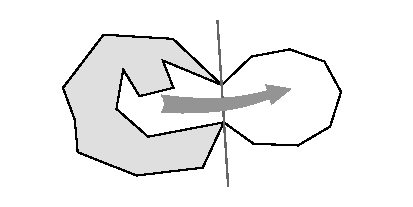
\includegraphics[scale=1.12]{img/carthage}
}
\end{tabular}\end{center}
\end{frame}

\begin{frame} \frametitle{2020-7-5B}
\usl{Найдите наибольшее натуральное число $n$ такое, что существует набор из $n$ различных простых чисел, сумма любых трёх чисел из которого является простым числом.}

\begin{itemize}
	\item из всех простых только 3 делится на 3;
	\item если у простых $p_1, p_2$ и $p_3$ одинаковые остатки от деления на 3, то $p_1+p_2+p_3$ делится на 3;
	\item поэтому нельзя брать более двух чисел с одинаковыми остатками;
	\item лучший вариант для нас $p_1, p_2$ с остатком 1 и $p_3, p_4$ с остатком 2.
\end{itemize}

\end{frame}

\begin{frame} \frametitle{2020-7-10C}
\usl{Один радист передал другому сообщение: «Всё очень плохо, вокруг сплошная слякоть». Каждый следующий радист передавал дальше сообщение, которое начинал со слов «Привет, друг!», а затем дважды повторял текст сообщения, которое получил. Из скольки слов состоит сообщение, отправленное $n$-ым радистом?}

	$$2 \cdot \ll 2^{n+2} - 2 \rr + 2 = 2^{n+1+2} - 2.$$

\begin{itemize}
	\item Чтобы получить ответ, нужна доля интуиции;
	\item Доказательство по индукции.
\end{itemize}

\end{frame}

\section[Методика]{What to Teach Kids}

\fram{Навыки участника}{
	\begin{enumerate}
		\item {\bf Можно ли?} \\
			\qquad Да — привести пример\scolon\\
			\qquad Нет — {\bf доказать}, что нельзя.
		\mitem {\bf Всегда ли?} \\
			\qquad Да — {\bf доказать} это\scolon\\
			\qquad Нет — привести контрпример.
	\end{enumerate}}

\fram{Ещё навыки участника}{
	\begin{enumerate}
		\setcounter{enumi}{2}
		\item Умение строить отрицания: \\
		\qquad {\bf не} (для всякого…) = существует такой, что ({\bf не} …)\scolon\\
		\qquad {\bf не} (существует такой, что …) = для всякого ({\bf не} …).
		\mitem Что такое доказательство — \\
		\qquad это обоснованное на каждом шаге рассуждение о том, почему \\
		\qquad верно так и никак иначе. Это {\bf не} приведение одного примера, \\
		\qquad для которого выполняется то, что должно быть верно всегда.
		\mitem Получаемый результат $\gg$ изученные алгоритмы и клише.
	\end{enumerate}
}

\fram{Подготовка к олимпиаде}{
	\begin{enumerate}
		\item Если начнёте тренировать детей для олимпиад — то быстро вырастете из МНС (оно и хорошо).
		\mitem Если начнёте специально тренироваться для МНС — есть профильный вариант; условия меняются год от года.
		\mitem Если просто учите класс — смотреть на то, чтобы дети находили результат и грамотно его обосновывали.
		\mitem Мы бы хотели, чтобы участники умели {\it писать} и {\it высказывать сложную мысль}.
	\end{enumerate}}


\section[Конец]{Fin}

\def\fitem#1#2{\textcolor{hard}{\small (#1)}~~#2 \medskip \\}

\begin{frame} \frametitle{Заключение}

\textcolor{hard}{Направления, которые мы обсудили сегодня} \medskip

\fitem{1}{Задачи, вдохновлённые реальными явлениями}
\fitem{2}{Конструктивные задачи}
\fitem{3}{Ужасный гадкий аккуратный подсчёт}
\fitem{4}{Задачи, где важно прочитать условие}
\fitem{5}{Сложные задачи для опытных детей \vspace{6mm}}

\hrule
\begin{center}
	{\LARGE Спасибо за внимание!} \smallskip \\
	{\footnotesize \textcolor{hard}{($*$)\quad}
		\url{mathnonstop.ru}
		\phantom{($*$)\quad}}
\end{center} \vspace{2.4mm}
\end{frame}

\end{document}
